\documentclass[12pt]{article}
\usepackage{amsmath}
\usepackage{graphicx}
\usepackage{hyperref}
\usepackage[latin1]{inputenc}
\usepackage{verbatim}

\title{PyCon XIV Gliwice, Poland | programming challenges}
\author{Amsterdam Standard}
\date{03/11/22}

\begin{document}
\maketitle

We've prepared few little coding puzzles in \textbf{Python} for You! Don't hesitate to tackle them. There might be some gadgets awaiting if You can accomplish them. Good luck.

\vspace{1cm}

\centering
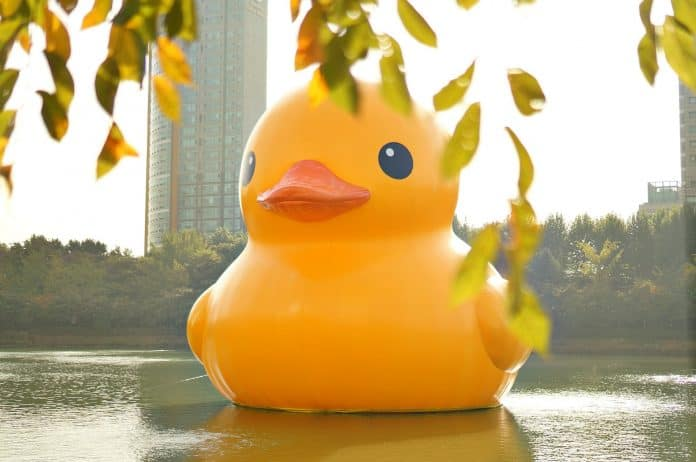
\includegraphics[width=10cm,height=10cm,keepaspectratio]{img/duck.jpg}

First task: Put all ducks in a row!

\vspace{1cm}
\begin{flushleft}
Few fellow ducks have visited us, perhaps You can remember them from old cartoon movies.
They arrived out of some order, but we must greet them according to it, to make sure no one is offended.

Switching to the programming world... We've prepared a little code snippet to begin with. We've categorized those ducks into 3 classes - \textbf{WeaklingDuck}, \textbf{Duck} and \textbf{SuperDuck} and created some objects.

\paragraph{Listing below is the entrypoint for You to complete the task.}

\begin{footnotesize}
\verbatiminput{src/ducks.py}
\end{footnotesize}
\vspace{1cm}

Here's output so far... not in order and the formatting could be better...
\begin{verbatim}
[<__main__.Duck object at 0x7f8ddfd0c730>,
 <__main__.SuperDuck object at 0x7f8ddfd0c790>,
 <__main__.SuperDuck object at 0x7f8ddfd0c6d0>,
 <__main__.WeaklingDuck object at 0x7f8ddfe29d30>]
\end{verbatim}

Your main goal is to sort them according to these specs (from highest priority to lowest):
\vspace{0.5cm}

\begingroup
\footnotesize
SuperDuck with speed boots
\succ

SuperDuck with any other Power
\succ

Duck
\succ

WeaklingDuck
\endgroup

\vspace{1cm}

Some rules:
\begin{itemize}
  \item you can use whatever module from \textit{stdlib}
  \item you can interfere with existing code - rearrange if needed!
  \item and don't forget - also make all the ducks greet themselves nicely!
  \item bonus: for shortest implementation or clever solution (or both)
  \item bonus: if you leave as much of existing code untouched, if possible
\end{itemize}

\end{flushleft}

\newpage


\includegraphics[width=10cm,height=10cm,keepaspectratio]{img/pumpkin.jpg}

Second task: Count all the pumpkins!

\vspace{1cm}
\begin{flushleft}

Halloween is the past tense already for this year, but we need Your help in cleaning out all the mess after the spooky party. We need to find out where are the hidden pumpkins - so we can be sure they will not start to rot and put a quite bad smell to the surroundings.

Again, translating it in the programmer's tongue...

We throw some text at you using generator - one line of fixed length at a time.

\begin{verbatim}
# some more code here
# ...

def main():
    for line in get_lines():
        # you code goes here

if __name__ == '__main__':
    main()
\end{verbatim}
\vspace{0.5cm}

The lines can contain word `PUMPKIN` (or parts of it). Your task is to count all the PUMPKINs according to these rules (just to make it a little bit more difficult):

\vspace{0.5cm}
Valid count scenarios:

\begin{itemize}
  \item somewhere in the line
  \begin{verbatim}
  fynp[;%)3mPUMPKIN"s~y4nkbx7m^&3b5@[,m^ny
  \end{verbatim}
  \item same as above, but reversed
  \begin{verbatim}
  bwk0\2l:<'n`dNIKPMUPm=j]5<byzNIKPMUPg5$3
  \end{verbatim}
  \item span over two lines, where one syllable is at the end of first line and the other one at the beginnig of next line
  \begin{verbatim}
  i75s7!yq&=![<?./j$$;1|\dl.>0s''1|3=2PUMP
  KIN#g65[/^u=a<>>u[{!6{(j8m:,h)<s1hi$@k[9
  \end{verbatim}
\end{itemize}

Invalid count scenarios:
\begin{itemize}
  \item at the beginning/end of the line
  \begin{verbatim}
  PUMPKINfynp[;%)3m"s~y4nkbx7m^&3b5@[,m^ny
  fynp[;%)3m"s~y4nkbx7m^&3b5@[,m^nyPUMPKIN
  \end{verbatim}
  \item when some other letter from the word is next to it (left or right)
  \begin{verbatim}
  ^o{(zyz"g<*a?UPUMPKINn{8,^=/tote30bkb*#2
  ^o{(zyz"g<*a?PUMPKINKn{8,^=/tote30bkb*#2
  \end{verbatim}
  \item \textbf{extra (*)} in some so called "trashy" lines, there are all letters from a word PUMPKIN, but in some they are out of order, if that's the case just skip them:
  \begin{verbatim}
  ;qqbkrMi+o.='je!<_m>}_'IvPt"9N^wU[PiK5c|
  \end{verbatim}
  but if they are in order (no matter how many other characters are interleaving them) - that's a count!
  \begin{verbatim}
  ;7Pa9%14U:ba$#m-4/x(M:P/bKIf6Nt<,~j1*2'(
  \end{verbatim}
\end{itemize}

EXAMPLE - for these lines the count is 2:
\begin{verbatim}
# c3!hny*,c5pbe3825rsh#m71i7{s^i$*o*g=ePUM
# PKIN/^+3m#(}j@2>8~nav\f>=PUMPKINs5:PUMPK
# IN*k$on#t.<p]pjia=35`at2@/PUMPKIN}g3l+*`
\end{verbatim}
\vspace{1cm}

The whole input can be found in \textbf{sample\_input.txt} file. And there is a little helper function that reads it line by line.
\vspace{0.5cm}

Bonus points for:

\begin{itemize}
  \item making it work if the letters forming a word, would be lowercase
  \item what if the word changed from 'pumpkin' to something else? will your code still work?
  \item try not to use `count`, `find`, `rfind` functions and `in` operator
\end{itemize}

\vspace{1cm}
Depending on some implementation details, for the input file You should get 52 or 60 (this is connected with extra case, but both are valid) as a number of pumpkins.

\vspace{1cm}
\hyperlink{example}{Sample input is at the end of this document.}

\end{flushleft}

\newpage

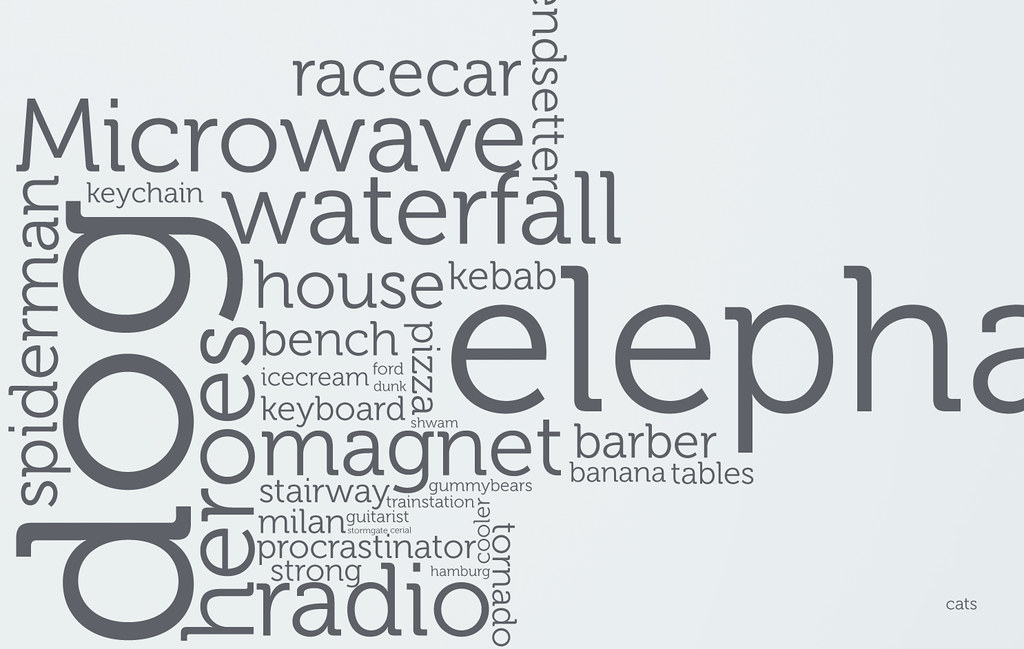
\includegraphics[width=10cm,height=10cm,keepaspectratio]{img/wordcloud.jpg}

Third task: First letter / last letter game!

\vspace{0.5cm}
\begin{flushleft}

After all the excitement of crazy halloween night and after all fellow ducks have left, we woke up to the harsh reality. To put a little smile back on our faces, we have decided to play some game called \textit{first letter last letter} so don't mind to join us!

The original game runs as follows:
one person thinks of a word e.g. \textit{elephan\textbf{t}}, then another person must find new word that starts with the last letter of the previous word e.g. \textit{\textbf{t}rip} and it continues...
\vspace{0.5cm}

There is an input file called \textbf{letter\_game.txt} that consists of surnames of important people in history of computing. Can you find the longest sequence of those that follow the rules of this game?
\vspace{0.5cm}

We will build a leaderboard - the person who will find the longest sequence wins!

\vspace{0.5cm}

Rules are:
\begin{itemize}
  \item use Python :)
  \item sequence must be found programmatically (with some logic) - no hardcoding!
  \item other than that anything goes!
\end{itemize}
\vspace{0.25cm}

The solution should be verifiable by the function below - it must return a 2-tuple containing positive number and a True and pass all the assertions:
\end{flushleft}

\begin{footnotesize}
\verbatiminput{src/letters.py}
\end{footnotesize}
\vspace{0.5cm}

We have some naive algorithm that has found some sequence of length 28 using randomness and recursion. Can You do better?
\vspace{0.5cm}

beck - knuth - hopcroft - tanenbaum - meijer - rossum - meyer - rivest - torvalds - stepanov - von-neumann - ng - gates - stroustrup - patterson - naur - raymond - dean - norvig - graham - musk - kleene - evans - schwartz - zuse - eich - hamming - gosling


\newpage

Here is the contents of a \textit{letter\_game.txt} file for third exercise:

\begin{verbatim}
lovelace
huffman
wolfram
gosling
codd
steele
felleisen
hoare
naur
zuse
mccarthy
berners-lee
turing
lamport
rossum
thompson
pike
sussman
sethi
karp
evans
karpinski
conway
eich
torvalds
norvig
church
musk
stepanov
ullman
babbage
friedman
floyd
shamir
chomsky
stroustrup
boole
raymond
fowler
meijer
matsumoto
liskov
kernighan
zuckerberg
beck
strassen
nakamoto
tukey
kay
kruskal
hejlsberg
wirth
stallman
stevens
perlis
knuth
rivest
odersky
sedgewick
shannon
graham
koenig
moore
hickey
warwick
gates
page
curry
minsky
lerdorf
adleman
amdahl
bell
dean
carmack
ng
hall
dijkstra
lecun
sutherland
leiserson
wall
meyer
peyton-jones
wozniak
hopper
ritchie
hopcroft
von-neumann
iverson
hamming
bellman
booch
schwartz
backus
tanenbaum
romero
kleene
hollerith
petri
aho
patterson
brin
russell
\end{verbatim}

\newpage

\hypertarget{example}{Here is an excerpt of \textit{sample\_input.txt} for second exercise:}

\begin{verbatim}
,081:c,9g*?}lcp)t7,e0(%|j:dt3\yn-4<!#5o7
q#PU>Mi%6.;Pd""{!0ju0z5u_s'c6*x8#KIjN4_:
yoP^/\_k}g('&raUdMPk[}.2eKhqI;"2@N\&<6g=
y>fzPmI3<2ujc.K-$qn-y6aU+6)m=PNm&/M"80r@
zf5b92|*php05l9"p_v|k++de6d,,!)(!l%hPUMP
KIN!}`m>c{qiiPUMPKINe/+i]i*}`%!zp*<b>NIK
PMUP0&vjp^^hp0a3$~_8n'4:gpw#,2~pr5f2^>6>
g|,r;)a.4v9`e-/+s~9x==z~rpl1=v13@t4.zsai
yh:<rPU+*M?0wx:`d<>l(x9{@qjvtvo&Pg+~KIN&
4[t`02;IU,Kdf-w"x,_ye;q.t$7%(mPN/=P9M5m\
<l6e0yng;PUMPKINv-$&g$b(j")-b4s(|i-.^vf7
gsP~7U5[M\4PjKs`]I';i&|2=\{}N[:!|0eg]:@=
\,([>age#p;ao?o&}6k^\&v1!o)~'i[r_vk7`_-8
#[55u;z$gq/f<s+g)3]xPUMPKIN!0,o-PUMPKIN#
_m=63=(ug1[-k\>}cg{l}PUMPKINik>hval&by@f
m:(l}%]d})8s1p}|ks,[1`d@,)t\e##"o>a-:|#e
:;kP!l+t5Ur<M]Pz_p:qa?rK\7,!>`|w7sv`9I.N
;}mz6;,]qwnc-`,h;78&8cmi~>PUMPKINzl*3j'!
1.@c"o+"8uxx96a/.jb)vp]f#&=_xf7vve]8ur8r
sz2>NIKPMUP.|r^!!?a&.x:.e+NIKPMUPPUMPKIN
N)@I%($o,P,a?f3M"9K|r&rvm34edPU+*g<~}/cc
ep7#e=m{5lbn,s.84/c<[[_>jx]4\2ui|bf/ukw(
dmky)44aj0u_$y24el0h(h''*c{gPUMPKIN>,;]>
nw09t|x-g2oh%NIKPMUP(%h=!0'+fc-u.0`>_%e@
\end{verbatim}

\thispagestyle{empty}
\vspace{3cm}
For more info about us, please visit our page @ LinkedIn
\url{https://pl.linkedin.com/company/amsterdam-standard}

or email us directly:
\href{mailto:info@amsterdamstandard.com}{Info @ Amsterdam Standard}!

\end{document}
